\chapter{Metodologia}
\label{cap:03}

Descrever metodologia, materiais e métodos utilizados no estudo, bem como os procedimentos experimentais realizados, nesta etapa será descrito vários assuntos sobre os passos a serem realizados iniciando com o levantamento dos dados, para uma analise e estudo posteriormente analisando todos os processos que são realizados, afim de iniciar o desenvolvimento.


\begin{figure}[ht]
    \caption{Passos feito na plataforma miro}
    \centering
    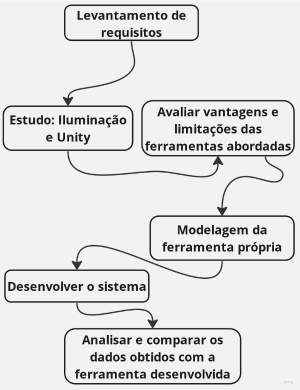
\includegraphics[scale=0.2]{imagens/Diagrama.jpg}

    Fonte: Feito pelo autor
    \label{fig:diagrama}
\end{figure}

Serão discutidos os principais passos estabelecidos para a execução completa do projeto idealizado, conforme ilustrado na Figura \ref{fig:desenvolvimento}.

\begin{figure}[ht]
    \caption{Passos feito na plataforma miro}
    \centering
    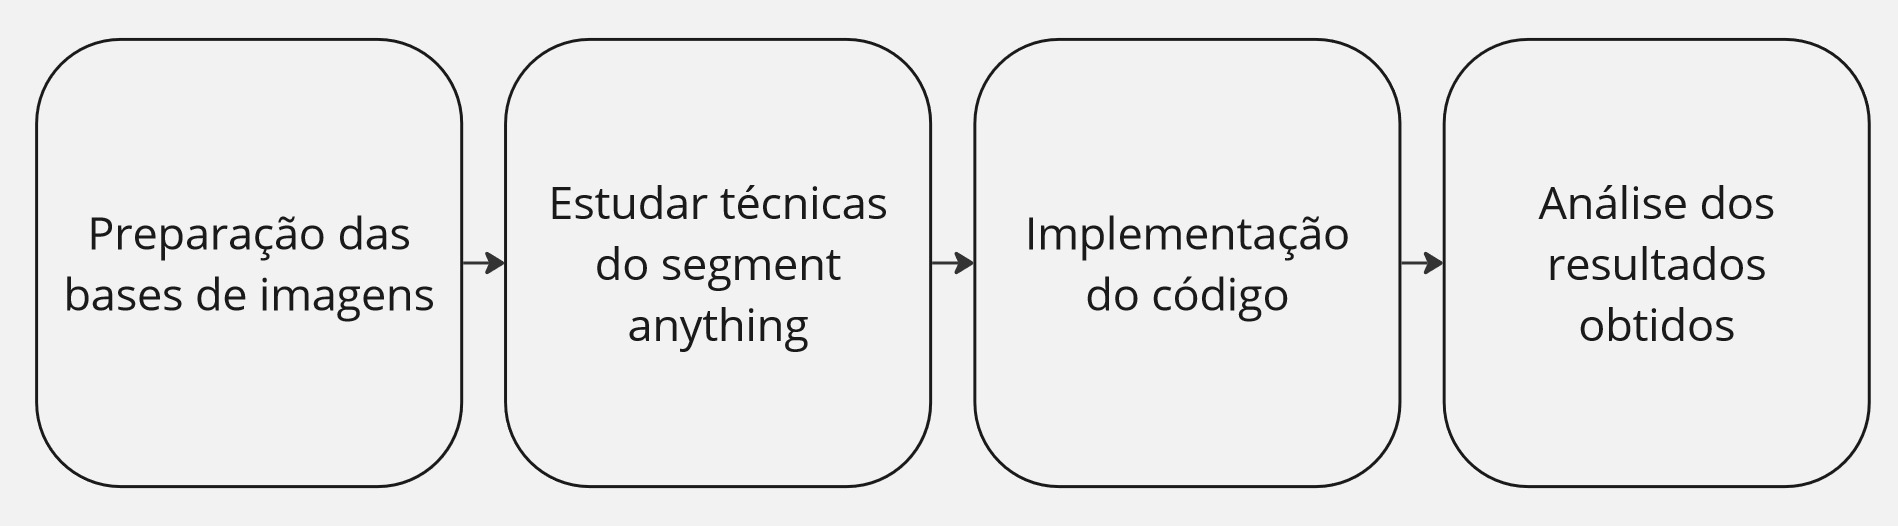
\includegraphics[scale=0.2]{imagens/progresso_desenvolvimento.jpg}

    Fonte: Feito pelo autor
    \label{fig:desenvolvimento}
\end{figure}

Como mostrado o diagrama foi elaborado utiliza duas cores distintas para representar o estado de cada fase do processo: verde, indicando as etapas em andamento; e vermelho, para aquelas ainda não iniciadas. As fases não iniciadas foram postergadas devido a dificuldades técnicas encontradas ao longo do desenvolvimento, as quais exigem uma análise mais aprofundada e a reformulação de estratégias para assegurar a eficiência e adequação da solução proposta.

\section{Levantamento de Requisitos}

Nessa sessão será abordado a pesquisa qualitativa feita a partir da ferramenta \textit{Relight} que usa de um algoritmo para identificação de camadas em uma imagem, assim, quando a imagem é colocada na ferramenta ela faz um mapeamento das áreas altas e baixas para criar as camadas, por esse motivo as camadas que são denominadas como mais alta recebe mais luz do que as mais baixas.

Porém a ferramenta tem uma funcionalidade a mais onde é possível definir em que nível está a luz, fazendo com que a iluminação do objeto possa vir das camadas mais a baixo para as camadas acima, está ferramenta com a luz funciona como um pincel de adicionar em softwares de pintura, pois ela recebe a luz já existente na foto e complementa por cima com a luz própria, podendo ser de qualquer cor.

A seguir será mostrado na tabela, onde terá a avaliação qualitativa referente a vários tipos de imagens testadas a partir da ferramenta, que para efeitos deste trabalho serão utilizados os valores de alta resolução como acima de 720 pixels, média resolução entre 720 e 256 pixels e baixa resolução abaixo de 256 pixels, retratado na tabela \ref{tab:desempenho_imagens}.

\begin{table}[h!]
    \centering
    \begin{tabular}{|l|l|l|l|}
    \hline
    \textbf{Imagem}        & \textbf{Alta Resolução} & \textbf{Média Resolução} & \textbf{Baixa Resolução} \\ \hline
    \textbf{Objetos}       & Funciona                & Funciona                 & Restrição                \\ \hline
    \textbf{Humanos}       & Funciona                & Funciona                 & Restrição                \\ \hline
    \textbf{Paisagens}     & Funciona                & Problema                 & Problema                 \\ \hline
    \end{tabular}
    \caption{Avaliação qualitativa da ferramenta}
    \label{tab:desempenho_imagens}
\end{table}

Nessa tabela, foi adotado três categorias para descrever o funcionamento: Funciona, Restrição e Problema.
A primeira categoria é utilizada para descrever que a imagem utiliza se comportou de forma correta, Restrição é a categorização para as imagens que funcionam mas em alguns casos ou áreas da imagem geram problemas, já a categoria Problema indica os casos onde a luz não reconhecia as formas de maneira correta.

\section{Estudo: Python e suas bibliotecas}
Nesta seção, será abordado sobre as diferentes bibliotecas estudadas para que a análise pudesse ser feita com o melhor aproveitamento da linguagem.
será mostrado também alguns tópicos referente ao estudo do python como linguagem em geral.

Para iniciar o estudo das bibliotecas antes, deve se entender melhor sobre os ambientes do python como o ambiente virtual, além de estudar como é o funcionamento das IDEs com o ambiente python dá mesma forma.


\subsection{PyTorch}

Para o uso da SegmentAnything o pyTorch é uma das dependências cruciais, já que ele aborda todo o processamento usado por placas de video e sistemas integrados com maior facilidade. 
O estudo dessa biblioteca se faz necessário apenas para a instalação de seus softwares dependentes como o uso do NVIDIA CUDA entre outros sistemas terceiros para o funcionamento do Segment Anything.

\subsection{Scikit-image}

O Scikit será extremamente necessário para a análise dos recursos e resultados obtidos, pois é com ele que conseguimos facilmente gerar as estatísticas como o MSE por exemplo.
Não apenas isso mas o estudo dessa ferramenta deve vir análoga ao estudo dos métodos de estimativa comparando duas imagens.

\subsection{OpenCV}

O OpenCV (\texttt{cv2}) será empregado para lidar com tarefas relacionadas ao processamento de imagens, como leitura, conversão e redimensionamento.
Ele será utilizado para ler as imagens a partir do disco (\texttt{cv2.imread}) e convertê-las entre diferentes espaços de cores para garantir a consistência de dados durante o processamento. Por exemplo, a função \texttt{cv2.cvtColor} será usada para converter as imagens do formato BGR para RGB, alinhando-as ao formato de cores esperado pelo modelo de segmentação. Além disso, o OpenCV será usado para redimensionar as imagens (\texttt{cv2.resize}) a fim de assegurar que elas possuam o mesmo tamanho antes de realizar comparações e cálculos de correlação. Um dos métodos-chave será o cálculo da Correlação Cruzada Normalizada (NCC), que será realizado por meio da função \texttt{cv2.matchTemplate}. Esse método permitirá medir a similaridade entre a imagem segmentada e a imagem esperada, fornecendo uma métrica quantitativa para avaliar a precisão do processo de segmentação.

\subsection{Numpy}
No projeto, o \texttt{numpy} será fundamental para a manipulação eficiente de arrays multidimensionais, que representarão as imagens processadas. O \texttt{numpy} será utilizado para criar e gerenciar esses arrays, facilitando a realização de operações matemáticas e comparações pixel a pixel nas imagens. Por exemplo, a função \texttt{np.zeros} será utilizada para inicializar uma matriz de zeros que servirá como base para a imagem segmentada final na função de geração de máscara. Além disso, o \texttt{numpy} permitirá a execução de operações eficientes, como a comparação entre arrays de imagens para verificar a igualdade de pixels com a função \texttt{np.array\_equal}. As imagens serão normalizadas convertendo os valores de pixel para um formato de ponto flutuante, possibilitando uma análise mais precisa ao dividir os valores por 255.0.

\section{Estudo: Inteligência Artificial}
Nesse estudo será demonstrado algumas das partes que serão necessárias para a criação da análise posteriormente, 
inicialmente foi preciso uma serie de estudos sobre todas as possibilidades relacionadas as possíveis segmentações realizadas, 
a seguir cada tipo de segmentação será melhor explicada.

\subsection{Segmentação por mascara}
A segmentação por máscara utiliza um modelo para identificar e isolar regiões específicas dentro de uma imagem. 
O modelo gera uma máscara binária onde a região segmentada é representada por 1 e o fundo por 0.
 Este método é eficaz para separar objetos ou áreas de interesse em imagens, permitindo uma análise mais detalhada dessas regiões específicas.

\subsection{Segmentação por pontos de clique}
Neste método, o usuário seleciona pontos dentro da área que deseja segmentar.
É utilizo esses pontos como referências para definir os limites da região de interesse.
 A segmentação é então ajustada com base na localização desses pontos, oferecendo um controle mais preciso sobre as regiões segmentadas, especialmente em imagens complexas.

\subsection{Segmentação por caixa de delimitação}
Aqui, o usuário fornece uma caixa delimitadora ao redor do objeto ou área de interesse. 
O modelo então realiza a segmentação dentro dessa caixa. 
Esse método é útil para rapidamente identificar e segmentar objetos que podem ser facilmente contidos dentro de uma área retangular, facilitando a definição da região de interesse.


\subsection{Segmentação por texto}
A segmentação por texto permite ao usuário descrever a região ou objeto desejado em termos textuais. 
O modelo utiliza essa descrição para identificar e segmentar a área correspondente na imagem. 
Este método é útil quando a descrição do objeto é mais clara em palavras do que em detalhes visuais, oferecendo uma maneira eficiente de segmentar com base em descrições contextuais.


\subsection{Segmentação interativa}
Este método combina várias abordagens interativas, como pontos de clique e caixas de delimitação, permitindo que o usuário refine a segmentação com base no feedback contínuo. 
A segmentação inicial pode ser ajustada e melhorada conforme o usuário fornece mais informações ou faz ajustes na área segmentada, resultando em uma segmentação mais precisa e adaptada às necessidades específicas.


\subsection{Segmentação automática}
Na segmentação automática, é aplicado algoritmos de segmentação sem intervenção do usuário. 
O modelo usa padrões aprendidos para identificar e segmentar automaticamente os objetos de interesse na imagem. 
Esse método é ideal para processar grandes volumes de dados ou quando a segmentação precisa ser realizada de forma rápida e eficiente em cenários bem definidos.

\section{Procedimentos e Técnicas}

Para o desenvolvimento desta pesquisa, foram realizados testes preliminares explorando toda a capacidade do modelo Segment Anything (SAM), com o intuito de validar a eficácia dos processos envolvidos na análise de segmentação de imagens. Durante essa fase inicial, foi constatado que o tempo de processamento se mostrou elevado, mesmo em um sistema com hardware moderno. Como resultado, optou-se por não utilizar a tecnologia NVIDIA CUDA, uma vez que o uso intensivo de processamento pela GPU não seria imprescindível para o escopo do projeto.

Com essa decisão tomada, iniciou-se uma nova bateria de testes envolvendo diferentes tipos de imagens, abrangendo diversas categorias visuais, a fim de avaliar o potencial de segmentação do SAM em variados contextos. Os resultados foram, em sua maioria, satisfatórios, com o modelo demonstrando desempenho adequado na maioria dos casos analisados.

Posteriormente, iniciou-se o desenvolvimento de imagens específicas, criadas pelo autor em estilo pixel art, para validar a performance do modelo em situações de segmentação por cor. Essa etapa exigiu ajustes no código, especialmente no que diz respeito à manipulação das camadas e formatos das imagens, além da tipagem adequada em Python. Esse processo envolveu pesquisas extensivas e múltiplas tentativas até a obtenção de um resultado satisfatório na geração de grupos de cores a partir das imagens.

Com o sistema de segmentação de imagens em funcionamento, iniciou-se a etapa de criação manual das camadas de segmentação. O autor definiu como deveriam ser os resultados esperados da segmentação proposta pela IA, segmentando um conjunto de 50 imagens em estilo pixel art com base em cores específicas para realizar as análises. A partir desse ponto, foi possível aplicar métodos existentes para a comparação entre duas imagens.

Inicialmente, foi desenvolvido um método próprio, denominado pelo autor como "Método de Espalhamento". Esse método parte do canto da imagem e realiza uma varredura pixel a pixel ao redor de cada ponto analisado, comparando diretamente com o resultado esperado. Caso a cor do pixel na imagem gerada seja diferente da cor prevista no resultado esperado, era gerada uma pontuação negativa. Se as cores coincidissem, o método prosseguia, continuando a busca por outras colorações na imagem base.

\section{Avaliar vantagens e limitações das ferramentas abordadas}

O \textit{Relight} é uma ferramenta muito boa para processos de iluminação tanto para cenários como personagens, com uma boa modificação como profundidade, posição, cor e luminosidade, dando para o usuário a liberdade de dar personalidade as suas imagens.

Mas ainda existe várias limitações e elas que serão retratadas nessa seção, como foi visto na analise a cima na tabela é possível notar que quanto menor a imagem é, menos funcional ela passa a ser, por exemplo imagens em baixa resolução ou pixeladas começam a ter muitos problemas pois a luz não consegue distinguir os objetos na cena e muito menos paisagens pois com tantas cores perto uma das outras transforma a cena em uma desordem visual.

Além da ferramenta abordada acima existe também algumas outras opções no mercado para este tipo de processo, como o laigter mas que ainda se envolve em uma limitação, que é o mapa de normais em apenas uma camada, o laigter atual na imagem fornecida pelo usuário como retratado na figura \ref{fig:laigter}.

\FloatBarrier
    \begin{figure}[ht]
        \caption{Imagens retiradas do GitHub da ferramenta}
        \centering
        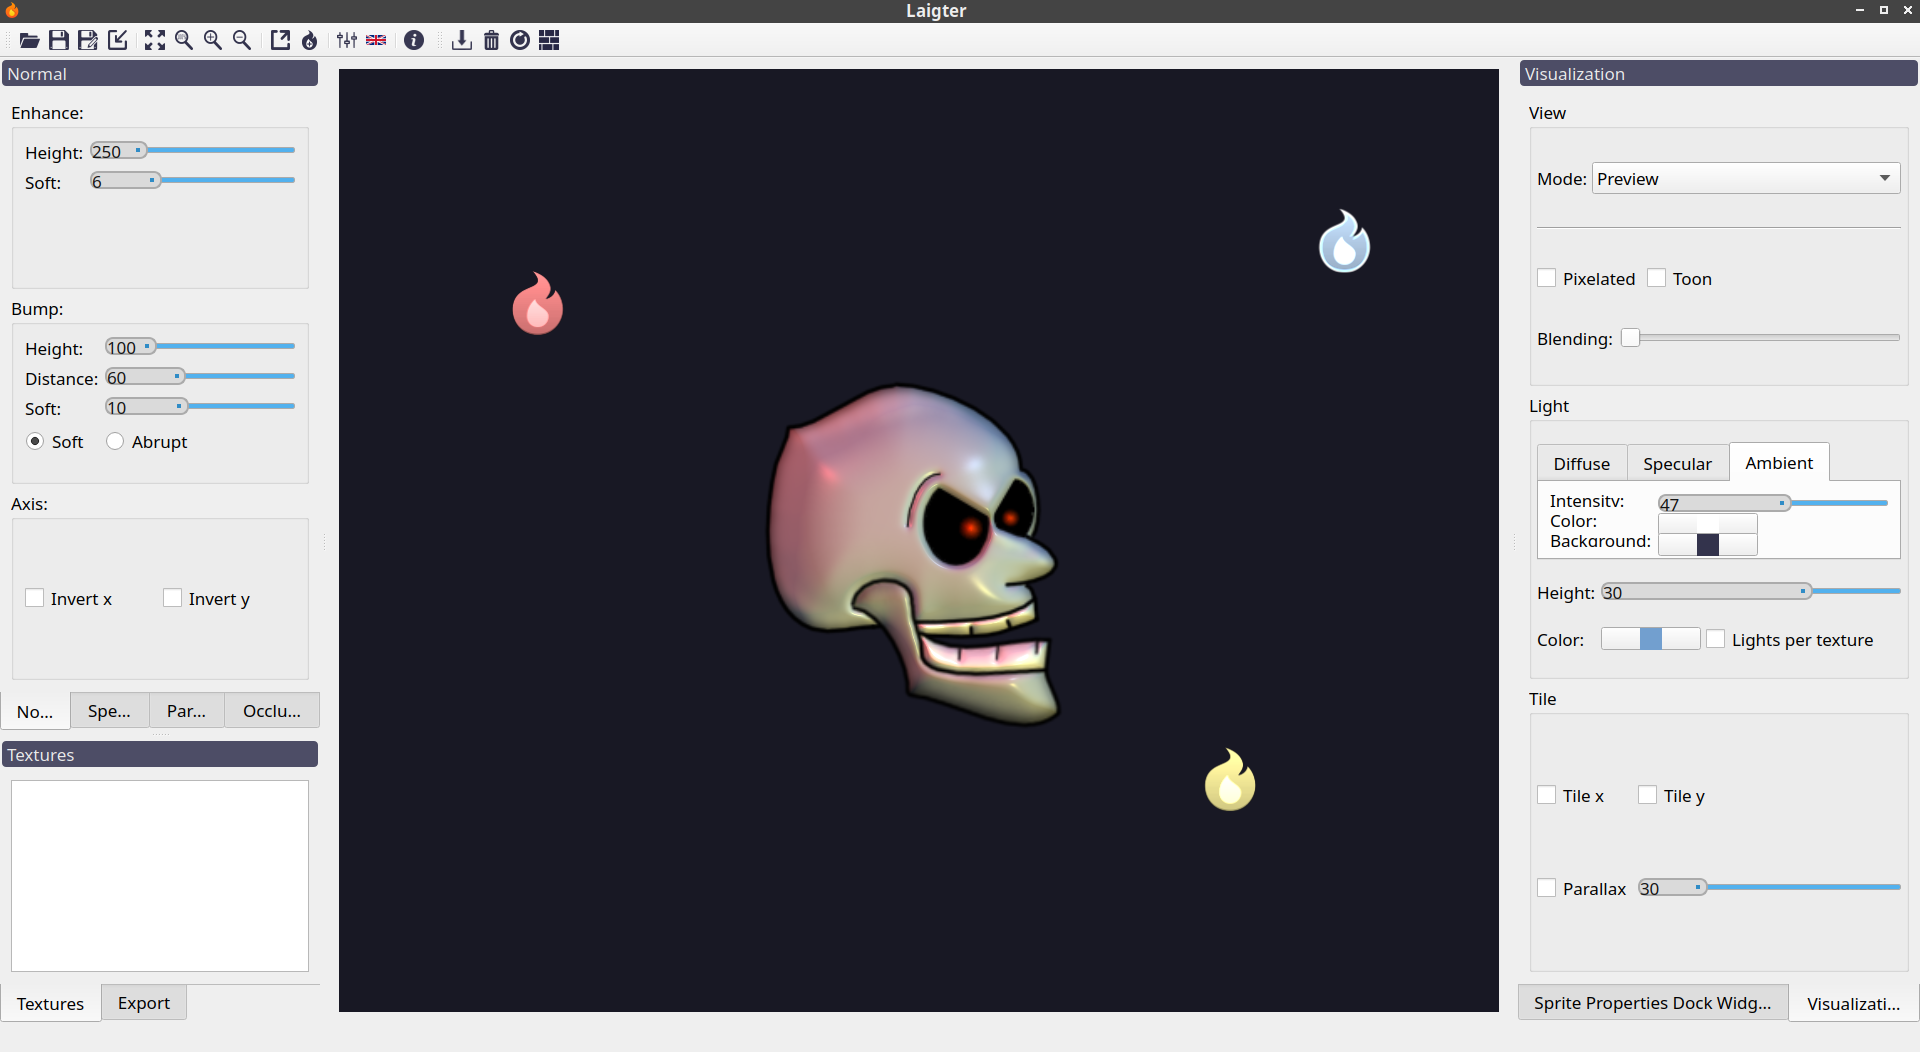
\includegraphics[scale=0.2]{imagens/laigter_example.png}
        \label{fig:laigter}
    \end{figure}
\FloatBarrier
    
\section{Modelagem da ferramenta}

Uma malha deverá ser criada por cima de toda a imagem e definir um inteiro para a profundidade, cada \textit{pixel} dá imagem deve receber uma profundidade como pode se observar na Figura \ref{fig:sketch}

\FloatBarrier
\begin{figure}[ht]
    \caption{Rascunho elaborado pelo autor}
    \centering
    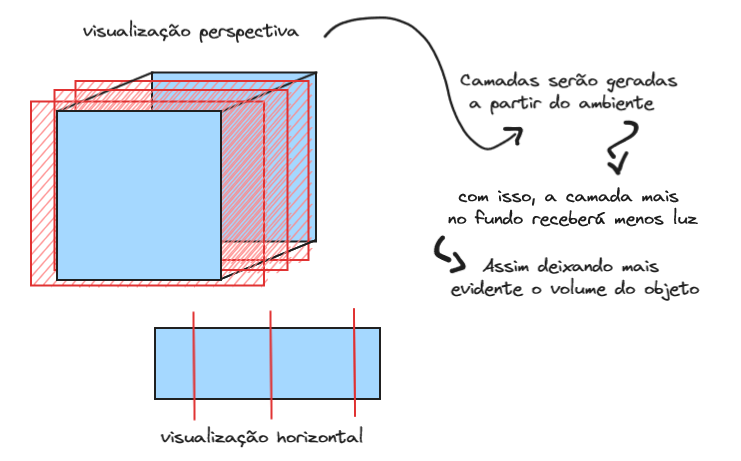
\includegraphics[scale=0.5]{imagens/Sketch.png}

    \label{fig:sketch}
\end{figure}
\FloatBarrier

Assim ele vai numerar toda a malha de \textit{pixels} na tela com números que podem ter uma variação maior dependendo do tamanho da imagem ( no caso de exemplo)

Será calculado de 1 a 9, mas com imagens imensas em alta resolução podemos pensar em usar de 1 a 100 ou até mais

Podemos pensar que dessa forma será possível utilizar essa profundidade para produzir uma luz pelas laterais ou pela frente e até atrás de elementos, sem perder sua funcionalidade até mesmo em imagens pequenas

Além disso, cada um desses valores definidos em cada \textit{pixel} da imagem, vão servir de referencia para criação de vários objetos, ele levará em consideração a distância e a variação de cor que foi atingida

Como por exemplo, se existir um objeto a frente da camada 1 até a 10 e um objeto atrás que está na camada 15, essa distancia de 5 camadas irá fazer o objeto dá frente se separar com o de trás transformando a cena com dois objetos ao invés de um

\section{Desenvolvimento do sistema}

Nesta seção será apresentado todos os processos em python realizados para a criação do código de análise dos dados criados e os já existentes realizados pelo autor, o desenvolvimento foi iniciado com a implementação das mascaras geradas pelo segment anything como mostra a figura \ref{fig:code1}.

\FloatBarrier
\begin{figure}[ht]
    \caption{Código elaborado pelo autor}
    \centering
    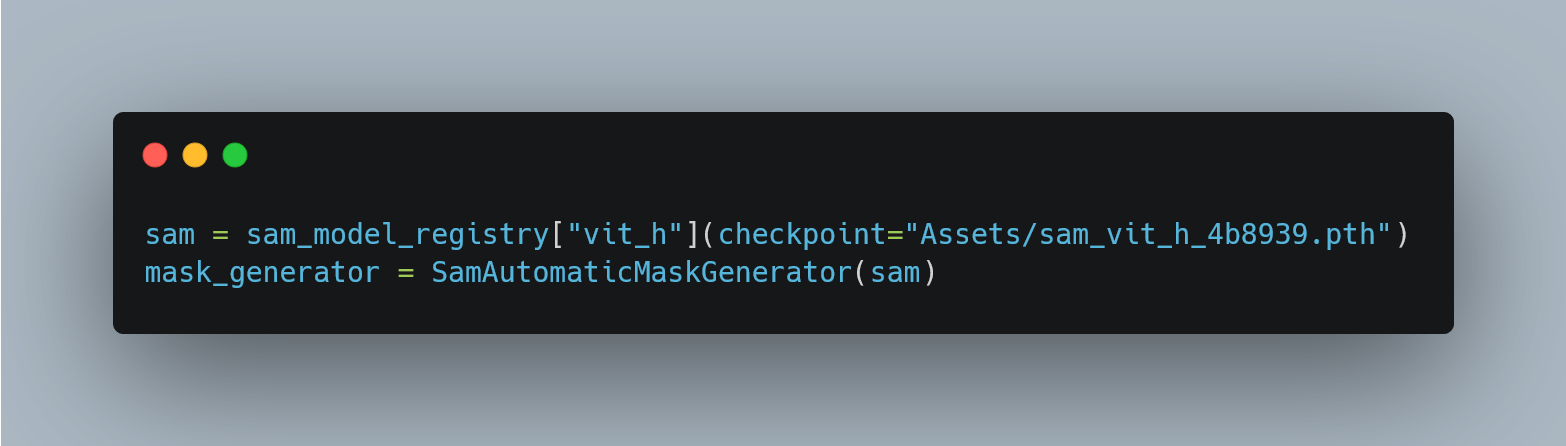
\includegraphics[scale=0.25]{imagens/code_part_one.png}
    \label{fig:code1}
\end{figure}
\FloatBarrier

Nesse processo a função faz o acesso do modelo que no caso utilizado foi o model vit h pesando 2.38 Gigabytes de memória, para essa função é possível a utilização de dois caminhos de processamento da imagem atual, o primeiro deles é utilizando a GPU de uma placa de vídeo o que em tese poderia diminuir o gargalo gerado nas CPUs e melhorar a velocidade em que é executado, logo após a geração das mascaras pelo SAM, o próximo passo é justamente iniciar a criação das mascaras manualmente.


Para essa etapa foi utilizado várias pixel artes retiradas do site: itch.io que tem grande parte da comunidade servindo \textit{assets} gratuitos para projetos pessoais ou jogos \textit{indie}, a execução dito foi realizada com uma visão humana para servir de referencia para os resultados gerados da inteligencia artificial, mas para as respostas do SAM não temos a geração de uma imagem em si mas de um \textit{array} de camadas criadas com cada segmento gerado, para isso se tornar uma imagem é necessário este código mostrado na figura \ref{fig:code2}.

\FloatBarrier
\begin{figure}[ht]
    \caption{Código elaborado pelo autor}
    \centering
    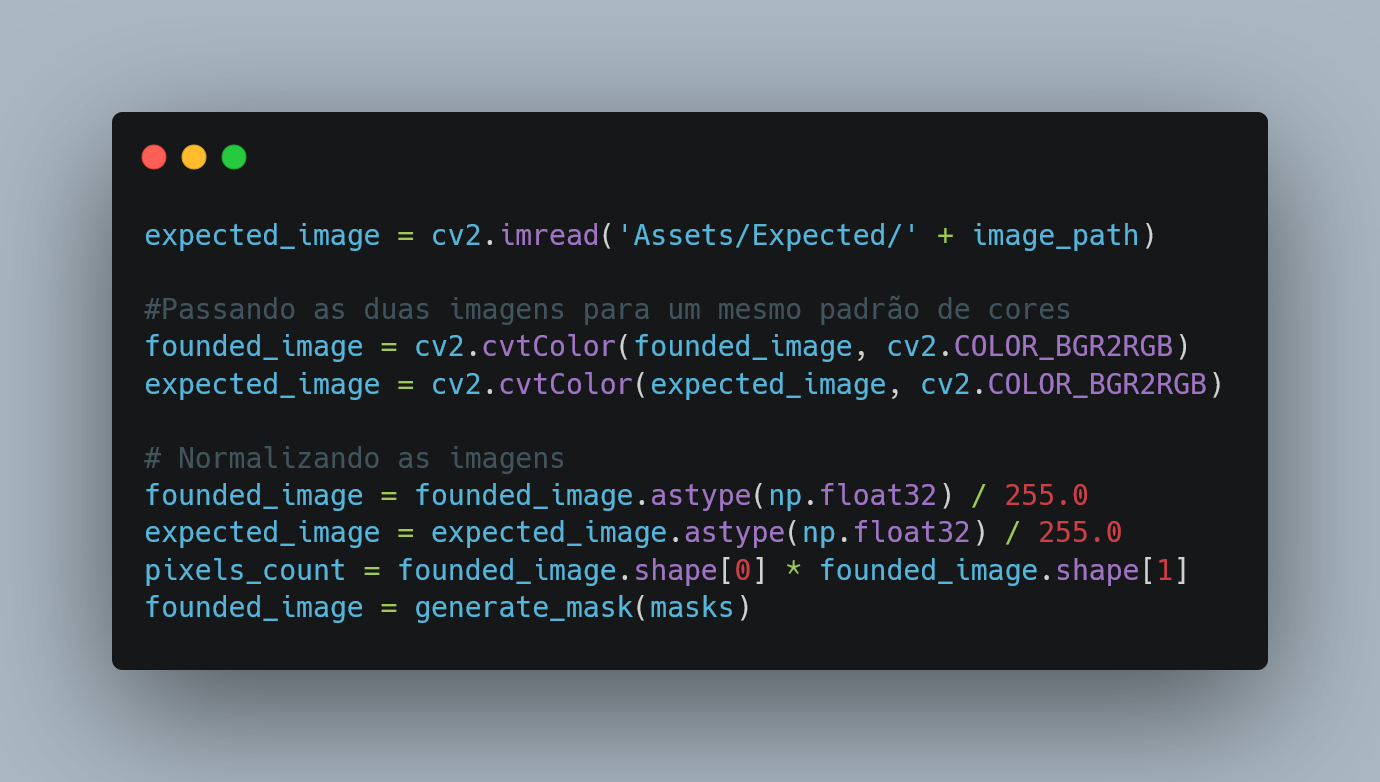
\includegraphics[scale=0.25]{imagens/code_part_two.png}
    \label{fig:code2}
\end{figure}
\FloatBarrier

Após os dois tipos de imagem já estarem preparados para a comparação é necessário a utilização de mais de um método de análise para compararmos e abrangermos mais pontos em comum sobre o resultado esperado, por isso é utilizado neste momento três tipos de análises, sendo duas delas configuradas pela biblioteca Scikit, a outra foi realizada pelo autor com a tentativa de gerar resultados diferentes dos métodos padrões.

O processo foi desenvolvido analisando a imagem pixel a pixel, começando no canto superior esquerdo, o primeiro pixel (coordenada zero). A varredura percorre cada linha da esquerda para a direita e, ao final de cada linha, passa para a próxima. Cada pixel possui duas referências: uma para a imagem original, segmentada pelo autor, e outra para a segmentação feita pela inteligência artificial (IA). Para cada pixel na imagem original, cria-se uma conexão com o pixel correspondente na imagem gerada pela IA, e o processo continua até que uma diferença de cor seja detectada entre os pixels correspondentes das duas imagens. Quando isso ocorre, o código verifica qual imagem apresentou a diferença primeiro; se a diferença for detectada primeiro na imagem original, o código marca essa mudança no grupo segmentado criando assim o inicio de uma nova conexão entre os pixels, mas, se a diferença aparecer apenas na imagem da IA, o pixel é marcado como incorreto, indicando um possível erro da IA, pois a imagem original ainda mantém a mesma cor. Ao final, a análise calcula a porcentagem de erros comparando o número de pixels incorretos com o total de pixels da imagem, todo este processo é feito nessa função do código-fonte como mostra a figura \ref{fig:code3}.

\FloatBarrier
\begin{figure}[ht]
    \caption{Código elaborado pelo autor}
    \centering
    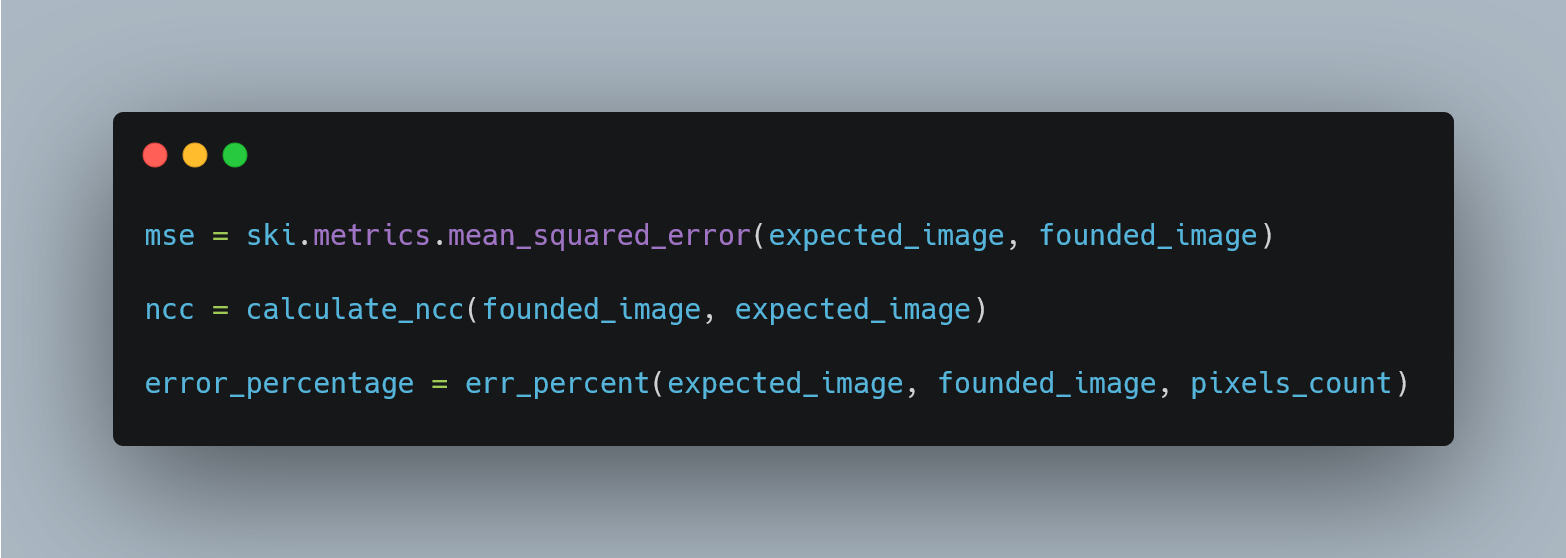
\includegraphics[scale=0.25]{imagens/code_part_three.png}
    \label{fig:code3}
\end{figure}
\FloatBarrier

Além da análise própria, também foram utilizados o método NCC e o MSE, que serão abordados a seguir. O primeiro deles, o NCC (Normalized Cross Correlation), é uma técnica usada para medir a similaridade entre imagens. Nela, utiliza-se geralmente uma imagem de referência e uma imagem-alvo; o índice de correlação varia de -1 a 1, onde valores mais próximos de 1 indicam alta similaridade, valores próximos de zero indicam baixa ou nenhuma correlação com a imagem de referência, e o valor -1 representa uma correlação inversa com a imagem. No entanto, o NCC não é vantajoso para casos em que há imagens complexas para analisar, o que é o oposto das imagens-alvo deste estudo.

O segundo método, o MSE (\textit{Mean Squared Error}), é uma técnica utilizada para avaliar a diferença entre duas imagens ao medir o erro médio entre os pixels correspondentes. O MSE calcula a média dos quadrados das diferenças de intensidade entre os pixels das duas imagens, gerando um valor que representa o grau de discrepância entre elas. Quanto maior o valor do MSE, maior a diferença entre as imagens comparadas; valores próximos de zero indicam alta similaridade. Esse método é simples e eficaz para medir discrepâncias, mas pode ser sensível a pequenas variações de pixel, sendo ideal para imagens onde os detalhes e as variações sutis são relevantes.

A combinação dessas três análises permite uma avaliação mais completa e detalhada da similaridade e discrepância entre as imagens, onde cada método contribui com uma perspectiva distinta. O cruzamento dos resultados oferece um panorama mais robusto, permitindo identificar falhas localizadas, medir a correlação global e quantificar as diferenças de intensidade de forma precisa. Essa integração facilita a obtenção de dados mais confiáveis e detalhados sobre o desempenho da segmentação, ampliando a compreensão sobre as sutilezas entre as imagens e fortalecendo a precisão das conclusões finais.

\section{Justificativa das Tecnologias a serem adotadas}

Para a criação da ferramenta de análise será utilizado o ambiente de desenvolvimento Visual Studio Code utilizando Python, foi optado este ambiente por sua praticidade com os diversos formatos de arquivos que serão utilizados ao decorrer do projeto. 
O python também servirá como única linguagem de programação para a ferramenta pela facilidade com a criação e uso das tecnologias de inteligencia Artificial que irá adiantar muitos dos processos necessários para a criação da análise.